\documentclass[landscape]{article}
\usepackage[paperwidth=252mm, paperheight=170mm, margin=0cm]{geometry}
\usepackage{tikz}
\usepackage{amsmath, amsthm, amssymb, mathtools, thmtools}
\usepackage{xcolor}
\definecolor{myBlue}{RGB}{173, 216, 230}
\definecolor{myGrey}{RGB}{200, 200, 200}

\usetikzlibrary{positioning, shapes.geometric, arrows}

% Define styles
\tikzstyle{node} = [rectangle, rounded corners, minimum width=1.5cm, minimum height=1cm, text centered, draw=black]
\tikzstyle{arrow} = [thick,->,>=stealth]

\begin{document}

\begin{figure}[h]
    \centering
    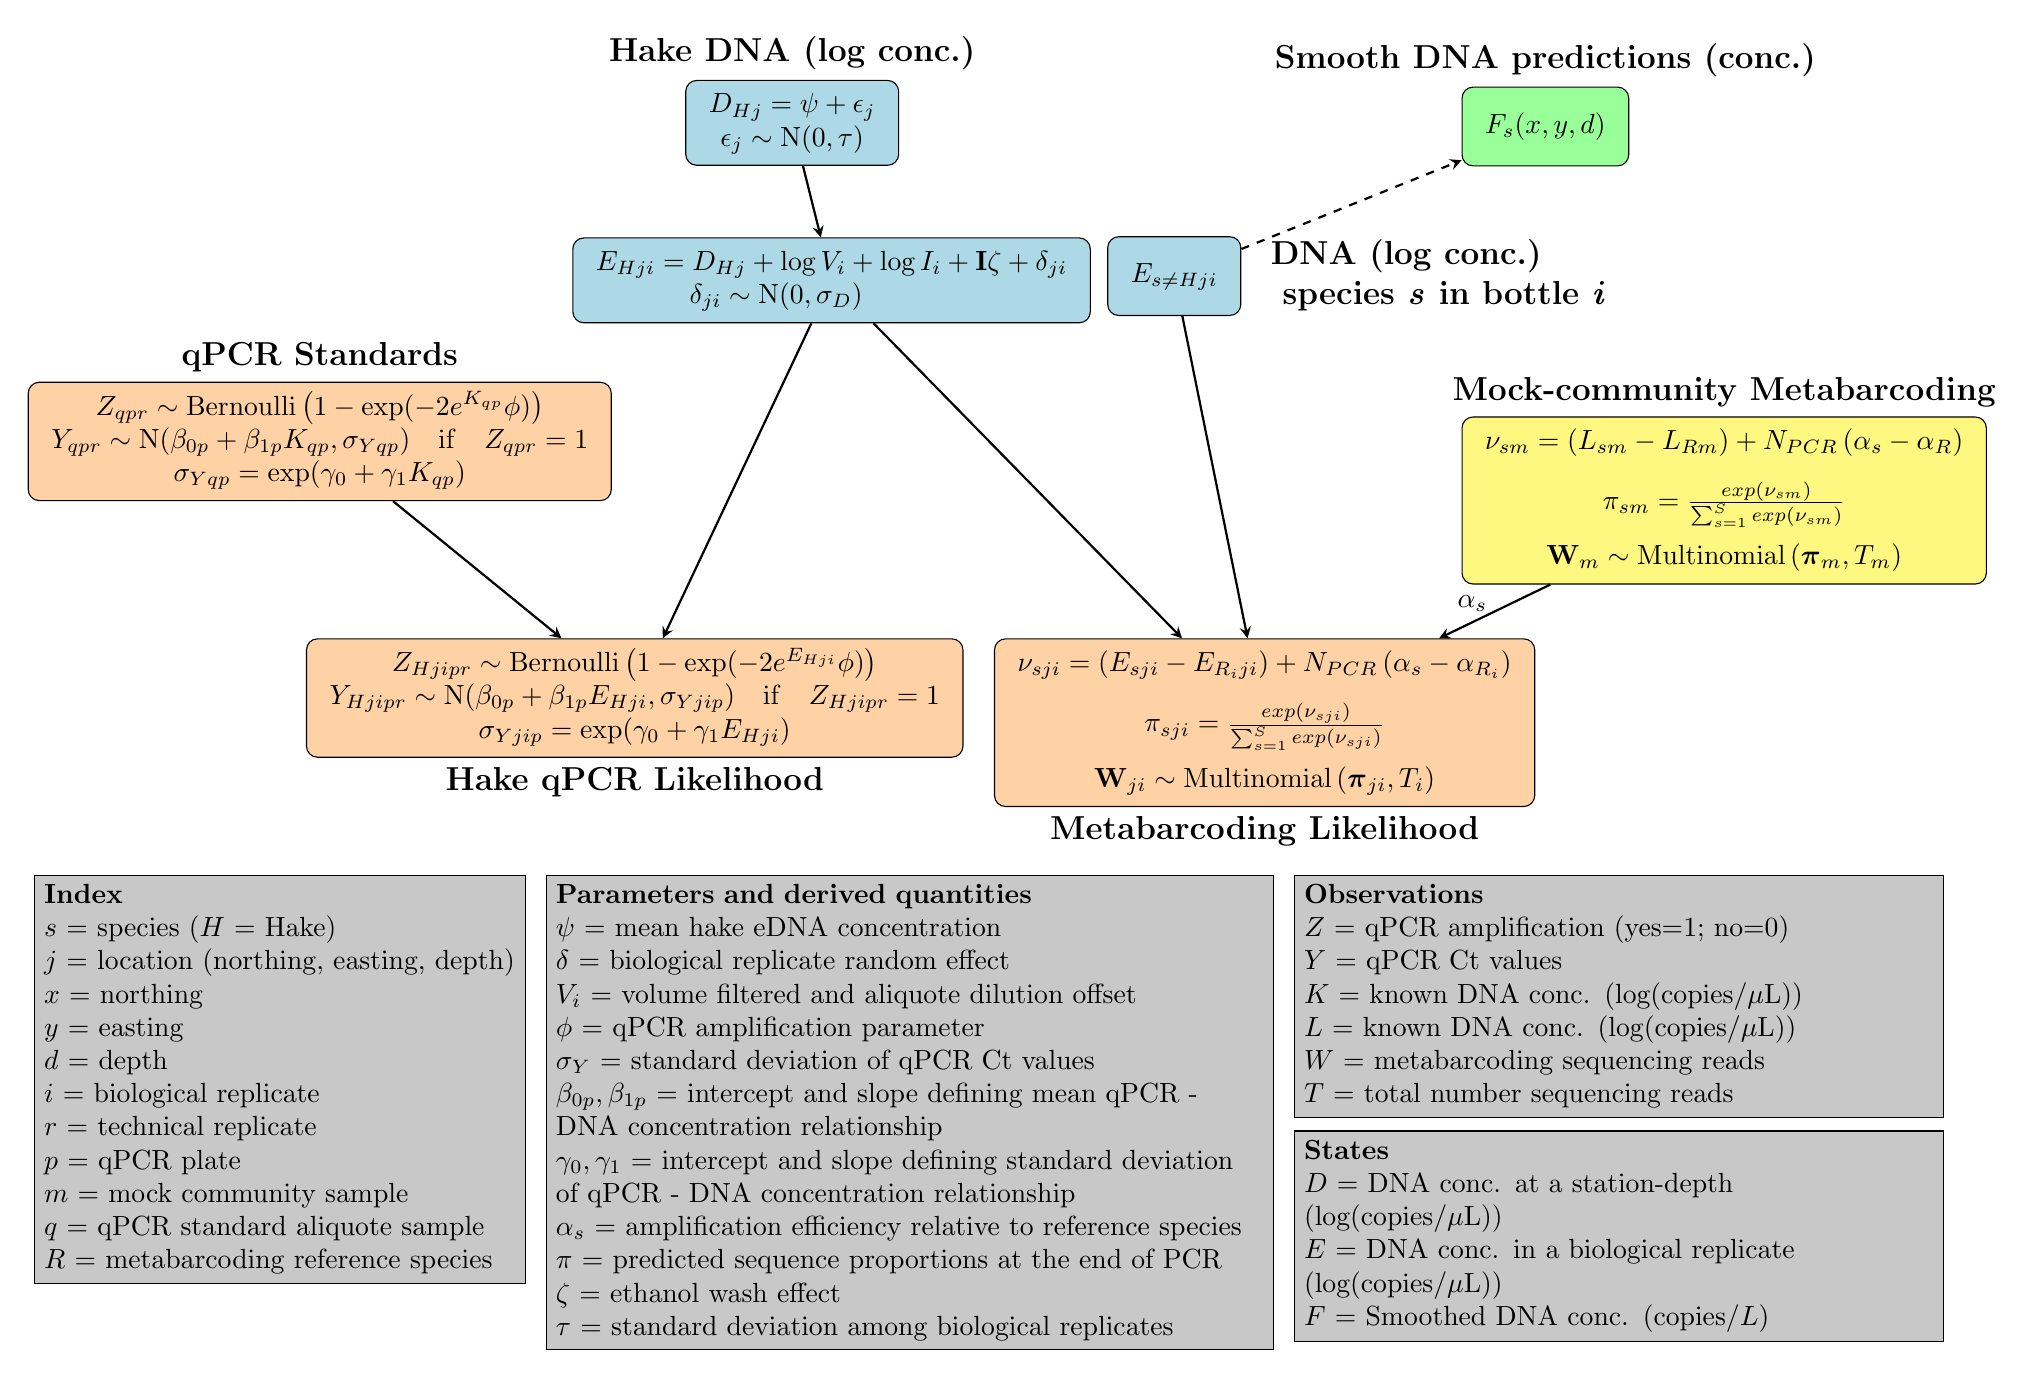
\begin{tikzpicture}[node distance=1.5cm]
        % Nodes
\node (qPCR_st) [node, fill=orange!35] at (-4,-2) {
    $\begin{array}{c}
       % \mu_{ik} = \beta_{0p} + \beta_{1p}  K_{i} \\
        Z_{qpr} \sim \mathrm{Bernoulli} \left( 1 - \exp(-2 e^{K_{qp}} \phi) \right) \\
        Y_{qpr} \sim \mathrm{N} (\beta_{0p} + \beta_{1p}  K_{qp} , \sigma_{Yqp}) \quad \mathrm{if}\quad Z_{qpr} = 1 \\
        \sigma_{Yqp} = \exp(\gamma_0 + \gamma_1  K_{qp}) \\
    \end{array}$
};
\node [above=of qPCR_st, yshift=-1.5cm, font=\large\bfseries] {qPCR Standards };
\node[anchor=south east] at ([xshift=5pt, yshift=-15pt] qPCR_st.south east) {};

\node (qPCR_en) [node, below=of qPCR_st, fill=orange!35]  at (0,-3) {
    $\begin{array}{c}
       % \mu_{ip} = \beta_{0p} + \beta_{1p} E_{Hi} \\
         Z_{Hjipr} \sim \mathrm{Bernoulli} \left( 1 - \exp(-2 e^{E_{Hji}} \phi) \right) \\
         Y_{Hjipr} \sim \mathrm{N} (\beta_{0p} + \beta_{1p} E_{Hji}, \sigma_{Yjip}) \quad \mathrm{if} \quad Z_{Hjipr} = 1 \\
         \sigma_{Yjip} = \exp(\gamma_0 + \gamma_1 E_{Hji})
    \end{array}$
};
\node [below=of qPCR_en, yshift=+1.5cm, font=\large\bfseries] {Hake qPCR Likelihood};
\node[anchor=south east] at ([xshift=5pt, yshift=-15pt] qPCR_en.south east) {};


\node (state1) [node, above=of qPCR_en, fill=myBlue] at (2,0){ 
% + \delta0_{ijdbt} 
% + \delta1_{ijdb}
    $\begin{array}{c}
        %\ln C_{ijdbt} = \psi_i + \ln D_{ijd} + \rho_{ijdbt} + \omega_{ijdbt} + \xi_{ijdbt} \\[8pt]
        %\ln C_{ijdbt} = \psi_i + \ln D_{ijd} + \rho_{ijdbt} + W_{ijdbt} + \xi_{ijdbt} \\[8pt]
        D_{Hj} = \psi  + \epsilon_j \\
        \epsilon_j \sim \mathrm{N}(0,\tau)
    \end{array}$
};
\node [above=of state1, yshift=-1.5cm, xshift=0cm, font=\large\bfseries] {Hake DNA (log conc.)};
\node[anchor=south east] at ([xshift=2pt, yshift=-15pt]state1.south east) {};

\node (state2H) [node, above=of qPCR_en, fill=myBlue] at (2.5,-2){ 
% + \delta0_{ijdbt} 
% + \delta1_{ijdb}
    $\begin{array}{c}
        %\ln C_{ijdbt} = \psi_i + \ln D_{ijd} + \rho_{ijdbt} + \omega_{ijdbt} + \xi_{ijdbt} \\[8pt]
        %\ln C_{ijdbt} = \psi_i + \ln D_{ijd} + \rho_{ijdbt} + W_{ijdbt} + \xi_{ijdbt} \\[8pt]
       E_{Hji} = D_{Hj} +  \log{V_i} +\log{I_i} + \mathbf{I}\zeta + \delta_{ji} \\
       		%\qquad \qquad \qquad \qquad 
		\delta_{ji} \sim \mathrm{N}(0,\sigma_D) \qquad \qquad
    \end{array}$
};
\node [above=of state1, yshift=-1.5cm, xshift=-1.3cm, font=\large\bfseries] {};
\node[anchor=south east] at ([xshift=2pt, yshift=-15pt]state1.south east) {};


\node (state2s) [node, right=of state2H, fill=myBlue]at (4.5,0.1) { 
% + \delta0_{ijdbt} 
% + \delta1_{ijdb}
    $\begin{array}{c}
        %\ln C_{ijdbt} = \psi_i + \ln D_{ijd} + \rho_{ijdbt} + \omega_{ijdbt} + \xi_{ijdbt} \\[8pt]
        %\ln C_{ijdbt} = \psi_i + \ln D_{ijd} + \rho_{ijdbt} + W_{ijdbt} + \xi_{ijdbt} \\[8pt]
        E_{s \neq Hji}
    \end{array}$
};
\node [right=of state2s, yshift=0.25cm, xshift=-1.25cm, font=\large\bfseries] {DNA (log conc.) };
\node [right=of state2s, yshift=-0.25cm, xshift=-1.1cm, font=\large\bfseries] {species \textit{s} in bottle \textit{i} };
\node[anchor=south east] at ([xshift=2pt, yshift=-15pt]state1.south east) {};


\node (metabarcoding) [node, below=of state2s, fill=orange!35]  at (8,-3) {
    $\begin{array}{c}
        \nu_{sji} = (E_{sji} - E_{R_iji} ) + N_{PCR} \left(\alpha_s - \alpha_{R_i} \right)  \\  [8pt]
        \pi_{sji} = \frac{exp({\nu_{sji}})}{\sum_{s=1}^{S} exp({\nu_{sji}})} \\ [8pt]
         \mathbf{W}_{ji} \sim \mathrm{Multinomial} \left( \boldsymbol{\pi}_{ji}, T_{i} \right) 
    \end{array}$
};
\node [below=of metabarcoding, yshift=1.5cm, xshift=0cm, font=\large\bfseries] {Metabarcoding Likelihood};
\node[anchor=south east] at ([xshift=4pt, yshift=-15pt] metabarcoding.south east) {};

\node (mock) [node,  right=of metabarcoding,fill=yellow!50] at (9,-2.75){
    $\begin{array}{c}
       \nu_{sm} = (L_{sm} - L_{Rm}) + N_{PCR} \left(\alpha_s - \alpha_{R} \right)     \\   [8pt]
       \pi_{sm} = \frac{exp({\nu_{sm}})}{\sum_{s=1}^{S} exp({\nu_{sm}})} \\ [8pt]
       \mathbf{W}_{m} \sim \mathrm{Multinomial} \left( \boldsymbol{\pi}_{m}, T_{m} \right) 
    \end{array}$
};
\node [above=of mock, yshift=-1.5cm, font=\large\bfseries] {Mock-community Metabarcoding};
\node[anchor=south east] at ([xshift=5pt, yshift=-15pt] mock.south east) {};

\node (spatial) [node, right=of state2s, fill=green!40] at (9,2){
    $\begin{array}{c}
        F_s(x,y,d) 
    \end{array}$
};
\node [above=of spatial, yshift=-1.50cm, xshift=0cm, font=\large\bfseries] {Smooth DNA predictions (conc.) };
\node[anchor=south east] at ([xshift=19pt, yshift=-4pt] spatial.south east) {};

        % Arrows
        \draw [arrow] (qPCR_st) -- node[pos=0.1, below] {} (qPCR_en);
        % \begin{array}{c}
        %     \phi, \\ \beta_0, \beta_1, \\ \gamma_0, \gamma_1
        % \end{array}$} (qPCR_en);
        \draw [arrow] (state1) -- node[midway, left] {$$} (state2H);
        \draw [arrow] (state2H) -- node[midway, right] {} (qPCR_en);
        \draw [dashed,arrow] (state2s) -- node[midway, right] {}  (spatial);
        %\draw [arrow] (state1) -- node[midway, right] {}  (spatial);
        \draw [arrow] (mock) -- node[pos=0.7, above] {$\alpha_s$} (metabarcoding);
        \draw [arrow] (state2H) -- node[midway, right] {$$} (metabarcoding);
        \draw [arrow] (state2s) -- node[midway, right] {$$} (metabarcoding);



% Legend: Parameters
\node (parameters) [rectangle, draw, align=left, below=of metabarcoding, text width=9cm, fill=myGrey] at (3.5,-6){
    \textbf{Parameters and derived quantities} \\
    $\psi$ = mean hake eDNA concentration \\
    %$\delta0, \delta1$ = offset from mean hake \\
    $\delta$ = biological replicate random effect \\
    %$\omega$ = ethanol wash effect \\
    $V_i$ = volume filtered and aliquote dilution offset \\
   % $\mu$ = mean Ct values of qPCR \\
    $\phi$ =  qPCR amplification parameter\\
    $\sigma_{Y}$ = standard deviation of qPCR Ct values \\
    $\beta_{0p}, \beta_{1p}$ = intercept and slope defining mean qPCR - DNA concentration relationship\\
    $\gamma_0, \gamma_1$ = intercept and slope defining  standard deviation of qPCR - DNA concentration relationship \\
    $\alpha_s$ = amplification efficiency relative to reference species \\
    $\pi$ = predicted sequence proportions at the end of PCR \\
    $\zeta$ = ethanol wash effect \\
    $\tau$ = standard deviation among biological replicates\\
};

% Legend: Subscripts
\node (subscripts) [rectangle, draw, align=left, below=of qPCR_en, text width=6cm, fill=myGrey] at (-4.5,-6) {
    \textbf{Index} \\
    $s$ = species ($H$ = Hake) \\
    $j$ = location (northing, easting, depth) \\
    $x$ = northing \\
    $y$ = easting \\
    $d$ = depth \\
    $i$ = biological replicate \\
    $r$ = technical replicate \\
    $p$ = qPCR plate \\
    $m$ = mock community sample \\
    $q$ = qPCR standard aliquote sample \\
    $R$ = metabarcoding reference species 
};

% Legend: Data
\node (data) [rectangle, draw, align=left, below=of subscripts, text width=8cm, fill=myGrey] at (12.5,-6){
    \textbf{Observations } \\
    $Z$ = qPCR amplification (yes=1; no=0) \\
    $Y$ = qPCR Ct values \\
    $K$ = known DNA conc. (log(copies/$\mu$L))\\
    $L$ = known DNA conc. (log(copies/$\mu$L))\\
    $W$ = metabarcoding sequencing reads \\
    $T$ = total number sequencing reads \\
};

% Legend: Data
\node (States of Interest) [rectangle, draw, align=left, below=of subscripts, text width=8cm, fill=myGrey] at (12.5,-9.25){
    \textbf{States } \\
    $D$ = DNA conc. at a station-depth (log(copies/$\mu$L)) \\
    $E$ = DNA conc. in a biological replicate (log(copies/$\mu$L)) \\
    $F$ = Smoothed DNA conc. (copies/$L$)\\
    };

    \end{tikzpicture}
    %\caption{Multifish DAG}
\end{figure}

\end{document}